\label{1_introducao}

A resolução de diversos problemas se dá na forma de algoritmos, de instruções bem definidas. No entanto, alguns algoritmos podem pedir inúmeras instruções até concluírem, o que pode até mesmo inviabilizar a solução encontrada. A Inteligência Artificial pode atuar sobre tais problemas de modo a interagir com o problema e aprender com ele a encontrar uma solução. Ótimos candidatos para esta tarefa são os chamados \emph{Algoritmos Evolutivos (AE)}.

Algoritmos evolutivos são aqueles que se baseiam nos princípios de evolução natural da Biologia, e são aplicados em um modo particular de solução de problemas: o da tentativa-e-erro. Tais algoritmos seguem um framework mais ou menos comum, atuante sobre diferente \emph{gerações} de um problema, por meio de mudanças e combinações de \emph{indivíduos} existentes numa \emph{população} \cite{eiben2003introduction}. Tal framework, conjuntamente com as ações evolutivas, pode ser visto na figura \ref{fig:evolution-framework}.

\begin{figure}[ht!]
    \centering 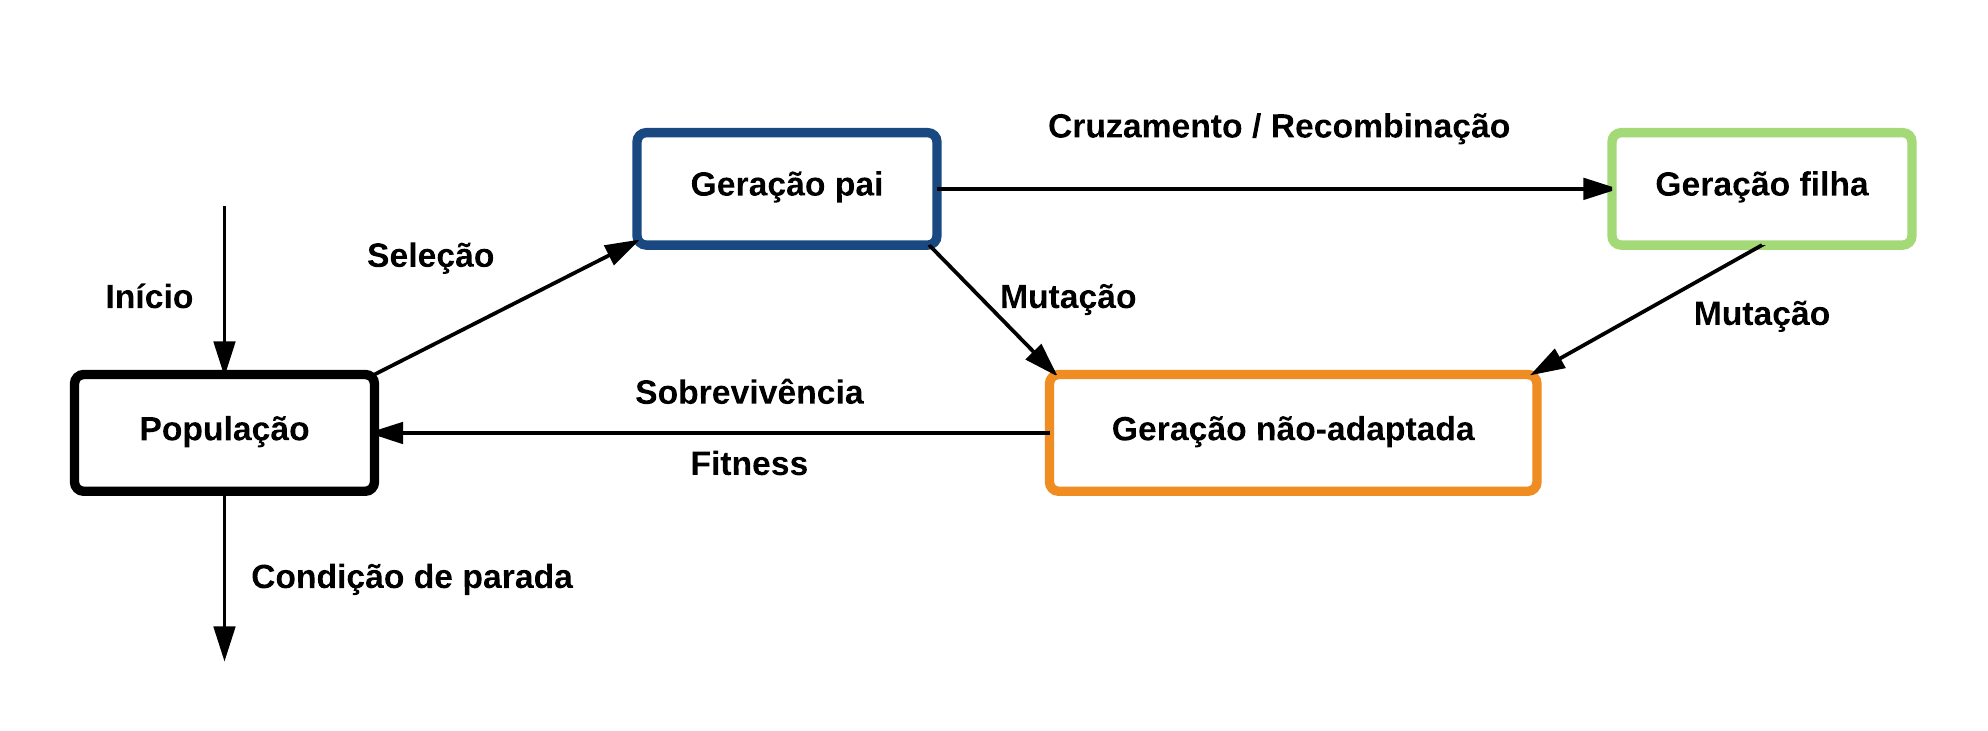
\includegraphics[width=1.0\textwidth]{evolution-framework.png}
    \caption{Framework de um algoritmo evolutivo.}
    \label{fig:evolution-framework}
\end{figure}

Cada indivíduo está tentando resolver o problema durante a execução do algoritmo evolutivo. A população contém estes indivíduos e é o alvo de interesse do processo evolutivo, e uma geração é a população que sobrevive após um ciclo de processos evolutivos do \ac{AE} sobre o problema. Similar ao processo evolutivo, seus componentes principais são as operações de variação (mutação e recombinação) e de seleção (seleção da geração pai e sobrevivência), chamadas aqui simplesmente de \emph{operações de evolução} \cite{eiben2011parameter}.

Este trabalho se utilizou de um grupo específico de Algoritmo Evolutivo, chamado de \textbf{Algoritmo Genético (AG)}. Um AG possui, como a menor estrutura de seus indivíduos, o \emph{gene}. Um gene costuma ter apenas duas propriedades: uma expressividade, normalmente associada a um valor numérico, e uma forma de mudá-la aleatoriamente.

Para um AG, a \emph{mutação} é uma mudança não controlada de um indivíduo feita a partir da mudança na expressividade de um ou mais genes. A \emph{recombinação} envolve a mistura de genes vindos de dois indivíduos que são cruzados. A \emph{seleção} envolve uma escolha a dedo dos melhores exemplares para cruzamento (a geração pai). A \emph{sobrevivência} envolve a rejeição de indivíduos que não estejam aptos o suficiente para resolver o problema. Tal aptidão é normalmente associada a uma função definida conjuntamente com o problema, chamada de \emph{função de fitness}.

\section{Motivação}

É difícil por si só garantir que um algoritmo evolutivo encontre boas soluções mesmo para os problemas mais simples, dada a natureza de sua implementação. Garantir uma execução eficiente do mesmo é fundamental.

\section{Objetivo}

Este trabalho propôs implementar um algoritmo genético capaz de resolver problemas determinados de diferentes complexidades e encontrar boas soluções após uma quantidade razoável de gerações.

\section{Abordagem}

Em termos de implementação, o AG deve ser tal que, uma vez aplicado sobre um problema e uma população, as gerações se desenvolvam automaticamente. O trabalho foi então dividido em 4 etapas:

\begin{enumerate}[label={[\arabic*]}]
	\item Escolha e implementação de problemas compatíveis com a aplicação do AE;
	\item Implementação do AG e de suas operações de evolução;
	\item Otimização das funções de mutação e recombinação;
	\item Análise de performance e coleta de dados.
\end{enumerate}

As primeiras duas etapas são interdependentes, e precisaram ser completadas primeiro. A terceira etapa funciona como a etapa de otimização do AG, e precisou ser tratada separadamente. A última etapa é uma etapa de análise, e foi encima dela que as conclusões foram feitas.

De modo a permitir a reutilização deste código em outros problemas, o AG foi feito de modo a ser compatível com mais de um problema. As ferramentas de análise e coleta de dados consideraram tanto métricas comuns da literatura quanto parâmetros específicos dos problemas abordados.

Optou-se por utilizar Python como linguagem principal do código feito para este trabalho.

%Para [1], como problemas diferentes se utilizarão do mesmo AE, as operações de evolução tiveram de representar o funcionamento do framework da forma mais essencial possível.

%Para [2], foi necessário não só deixar a população de um problema acessível ao AE, mas também dizer ao problema quão próxima de uma solução uma geração se encontra, ou quão melhor é um indivíduo frente aos demais. Tal escala foi trazida pelas funções de \emph{fitness}, definidas conjuntamente com o problema. Por exemplo, se um problema envolver o encontro das raízes de um polinômio, uma boa função de fitness para um indivíduo $x_k$ da população poderia ser definida por $|f(x_k)|$, indicando uma melhor solução quanto mais se aproximar de 0.

%Para [3], tendo tudo pronto, verificou-se a qualidade das soluções obtidas. Tais métricas são diferentes para cada problema, mas dependem do retorno feito pela função de fitness. Avaliou-se também como a função de fitness varia ao longo das gerações, tanto para os indivíduos quanto para a população.


%A etapa de implementação do AE 
%A proposta foi complexa, pois as três etapas são interdependentes. As etapas [1] e [2] pois as quatro etapas de criação do algoritmo são interdependentes. A etapa mais crítica foi a [1], que definiu o AE e o esqueleto de implementação de todas as outras etapas. As etapas [2] e [3] precisaram ter seus problemas/algoritmos bem definidos desde o início, para não atrapalharem o desenvolvimento em estágios avançados do trabalho. A etapa [4] precisou implementar diversas métricas ao longo de seu desenvolvimento, de modo a trazer as análises mais abrangentes possíveis para os problemas.

%Para a etapa [2], foram escolhidos os seguintes problemas:

%\begin{itemize}

%	\item \textbf{Problema OneMax Booleano\cite{giguere1998population}:} dado um conjunto de 100 bits iniciados em 0, o AE deve ser capaz de tornar todos os bits iguais a 1. A função de fitness avalia quantos bits estão iguais a 1 ao final de uma geração (quanto maior o valor, melhor, sendo 100 a solução ótima);

%	\item \textbf{Problema OneMax Real:} dado um conjunto de 100 variáveis reais iniciadas em 0, o AE deve ser capaz de tornar todas elas iguais a 1. A função de fitness aqui é semelhante à função do OneMax Booleano;

%	\item \textbf{O problema do Caixeiro Viajante \cite{applegate2011traveling}:} dado um conjunto de cidades e as distâncias entre elas, o AE deve ser capaz de descobrir qual o menor caminho que passa por todas as cidades e retorna à cidade original. A função de fitness avalia a distância percorrida a partir de um determinado percurso escolhido (quanto menor o valor, melhor). Sendo o problema NP-Hard, uma solução candidata à solução ótima também pediria um tempo 

%\end{itemize}

%Para a etapa [3], optou-se por escolher um algoritmo de tuning vastamente utilizado e comparado com outros em termos de performance para múltiplas literaturas \cite{eiben2011parameter, smit2009comparing}. Optou-se então pela implementação do algoritmo CMA-ES, o qual atua sobre o AE e sobre o problema até encontrar valores ótimos para os parâmetros de execução por meio de métodos estocásticos compatíveis com este tipo de problema \cite{hansen2006cma}.

%Dado também que era necessário analisar os problemas, o trabalho foi dividido em cinco módulos:

%\begin{enumerate}
%	\item Implementação do AE e de suas operações de evolução;
%	\item Implementação dos problemas e de suas funções de fitness;
%	\item Implementação do algoritmo CMA-ES para tuning do AE;
%	\item Implementação da função utilidade;
%	\item Execução completa do AE (precedida de tuning) e análises do AE a partir da função utilidade.
%\end{enumerate}

\section{Plano de Trabalho}
\label{sec:plano_trabalho}

Este trabalho foi planejado de forma que as etapas de otimização e análise do AE demorassem mais tempo. A validação dos resultados foi feita com base na literatura encontrada e nos resultados obtidos por algoritmos de código aberto (\emph{open source}) aplicados aos mesmos problemas.

\section{Organização do Trabalho}

\begin{itemize}
	\item \textbf{Capítulo 1:} Introdução
	\item \textbf{Capítulo 2:} Problemas Escolhidos
	\item \textbf{Capítulo 3:} Algoritmo Genético
	\item \textbf{Capítulo 4:} Otimização de Mutação e Recombinação
	\item \textbf{Capítulo 5:} Validação com Outros Trabalhos
	\item \textbf{Capítulo 6:} Conclusões e Trabalhos Futuros
\end{itemize}
